% ============================================================
% Predicting the Cost of Blocked Tracker Requests
% Target venue: IMC / PAM / PoPETs
% ============================================================

\documentclass[sigconf,nonacm]{acmart}

\usepackage{booktabs}
\usepackage{amsmath}
\usepackage{graphicx}
\usepackage{subcaption}
\usepackage{xspace}

\settopmatter{printfolios=true}

\newcommand{\numrequests}{3{,}490{,}824\xspace}
\newcommand{\numdomains}{3{,}723\xspace}
\newcommand{\numtrainrows}{2{,}443{,}576\xspace}
\newcommand{\numtestrows}{523{,}624\xspace}

\begin{document}

\title{Predicting the Cost of Blocked Tracker Requests\\from Pre-Response Features}

\author{James Han}
\affiliation{%
  \institution{Mozilla}
  \city{Toronto}
  \state{Ontario}
  \country{Canada}
}
\email{jhan@mozilla.com}

% \author{Tim Huang}
% \affiliation{%
%   \institution{Mozilla}
%   \city{Berlin}
%   \country{Germany}
% }
% \email{thuang@mozilla.com}

% \author{Manuel Bucher}
% \affiliation{%
%   \institution{Mozilla}
%   \city{Berlin}
%   \country{Germany}
% }
% \email{mbucher@mozilla.com}

% ============================================================
\begin{abstract}
% ============================================================

Firefox's Enhanced Tracking Protection blocks third-party tracker requests before any response is received, leaving the cost of what was blocked---transfer size, download duration, latency---structurally unknown.
We develop a per-request cost prediction model, scheduled for deployment to Firefox's 250 million daily active users, that estimates these costs from pre-response features alone.

Analyzing \numrequests tracker requests across \numdomains domains in the HTTP Archive, we find that within-domain transfer size variance spans three orders of magnitude, with the URL path as the primary determinant: the same domain serves both 93\,KB script bundles and 0-byte beacons.
This variance is invisible to domain-level lookup tables but predictable from URL structure.
XGBoost with Tweedie loss reduces transfer size MAE by 47.5\% over the best practical lookup table (3,466 vs.\ 6,597 bytes, 95\% CI [3,314, 3,627]) and outperforms even exact-path memorization on matched paths (1,346 vs.\ 1,448), demonstrating learned regularization beyond lookup.
Loss function selection dominates architecture selection: Tweedie outperforms squared error by 23\% on identical features.
The model generalizes across time (32.8\% improvement retained on a 3-month temporal holdout) and under correlated-browsing simulation (12.9\% weekly error vs.\ 36.4\% for the lookup table).
When aggregated to weekly totals, the model's estimate has 6.0\% median error---sufficient for user-facing display.

\end{abstract}

\keywords{web privacy, tracker blocking, cost estimation, Tweedie regression, URL embeddings}

\maketitle

% ============================================================
\section{Introduction}
\label{sec:intro}
% ============================================================

Firefox's Enhanced Tracking Protection (ETP) blocks third-party tracker requests identified by the Disconnect list~\cite{disconnectlist}, preventing advertising, analytics, and social tracking scripts from loading.
Firefox serves approximately 250 million daily active users, each of whom sees a privacy dashboard reporting how many trackers were blocked---but not the performance cost prevented.
Every blocked request is treated equally: a 258-byte tracking pixel from \texttt{bat.bing.com} counts the same as a 170\,KB JavaScript SDK from \texttt{googletagmanager.com}.

Quantifying the cost of blocked requests is a counterfactual estimation problem: the response was never received, so its size and timing are unknown.
The browser observes only the request URL, resource type, initiator, and HTTP metadata---features available before the block decision.
The response---transfer size, content type, download duration---is unobserved.

A natural baseline is a lookup table (LUT) mapping each (domain, resource type) pair to a historical median response size.
However, a single tracker domain serves resources of vastly different sizes: \texttt{googletagmanager.com/gtag/js} returns a 93\,KB script bundle while \texttt{googletagmanager.com/collect} returns a 0-byte beacon (Figure~\ref{fig:domain-example}).
We measure within-domain transfer size variance across \numdomains tracker domains and find a coefficient of variation exceeding 3$\times$ at the 75th percentile and 29$\times$ at the 90th, confirming that domain-level aggregation loses critical information.

\begin{figure}[t]
    \centering
    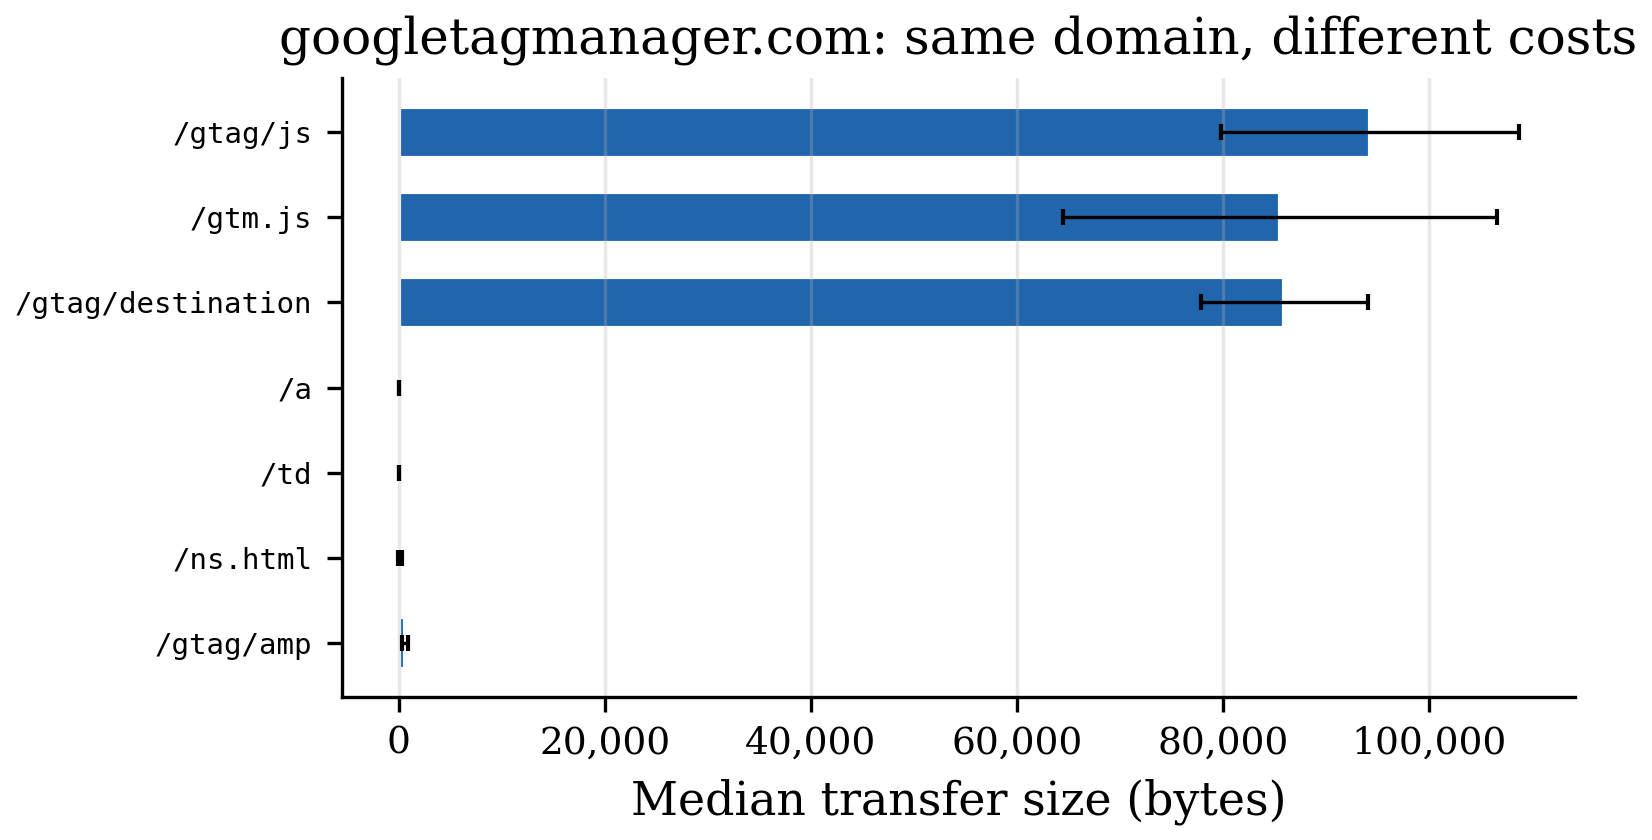
\includegraphics[width=\columnwidth]{figures/fig11_domain_example.pdf}
    \caption{Transfer size varies by orders of magnitude within a single tracker domain (\texttt{googletagmanager.com}). A domain-level lookup table conflates 90\,KB script bundles with near-zero beacon endpoints.}
    \label{fig:domain-example}
\end{figure}

A finer-grained path-level lookup table achieves lower per-request error when it has an exact match, but 75\% of unique URL paths in the test set are unseen in training, and the URL path space changes continuously as tracker SDKs evolve.
A model that generalizes from URL \emph{structure} rather than memorizing exact paths is required.

We formulate per-request cost prediction as supervised regression with a structural inference-time information gap.
The training set consists of completed tracker requests from the HTTP Archive~\cite{httparchive}, where both pre-response features and post-response labels are observed.
At deployment, the model predicts costs for blocked requests where only pre-response features exist.
Unlike domain-level cost estimation---which we show does not require machine learning (Section~\ref{sec:domain-level})---the per-request formulation has a genuine prediction gap: the response is structurally unobservable.

\paragraph{Contributions.}
\begin{enumerate}
    \item \textbf{Measurement finding.} We measure within-domain transfer size variance across \numdomains tracker domains and find that it spans three orders of magnitude (CV 0.94 at median, 3.0 at 90th percentile), with the URL path---not the domain---as the primary determinant. This variance is predictable from pre-response features, enabling per-request cost estimation rather than crude domain-level averages (\S\ref{sec:problem}--\ref{sec:data}).

    \item \textbf{Methodological finding.} For zero-inflated web response data, loss function selection dominates architecture selection: Tweedie loss outperforms squared error by 23\% on identical XGBoost features, while the gap across tree-based architectures is less than 5 points. Data-driven TF-IDF URL embeddings subsume hand-crafted regex features with a 17\% MAE reduction (\S\ref{sec:loss-ablation}--\ref{sec:feature-ablation}).

    \item \textbf{Generalization finding.} The model outperforms even exact-path lookup tables on paths with training matches (MAE 1,346 vs.\ 1,448), demonstrating that learned regularization across URL structures beats memorization. Per-request prediction noise cancels in weekly aggregation---including under correlated browsing patterns---producing estimates with 6.0\% median error (\S\ref{sec:baselines}, \S\ref{sec:aggregation}).

    \item \textbf{Negative finding.} Domain-level tracker cost estimation does not require machine learning. We diagnose a feature-space disjointness between labeled and unlabeled domain populations that explains a self-training null result and motivates the per-request reformulation (\S\ref{sec:domain-level}).
\end{enumerate}

% ============================================================
\section{Related Work}
\label{sec:related}
% ============================================================

\paragraph{Third-party web performance.}
The HTTP Archive~\cite{httparchive} crawls millions of pages monthly, storing per-request HAR data and Lighthouse audit results.
The Web Almanac~\cite{webalmanac2022} reports that the median page loads resources from 21 third-party domains.
\citet{pourghassemi2021adperf} developed adPerf, which instruments Chromium's activity trace to attribute CPU costs to individual ad scripts.
\citet{kontaxis2015tracking} measured Firefox's Tracking Protection, finding a 44\% median reduction in page load time and 39\% reduction in data usage on Alexa top-200 news sites.
The Ghostery Tracker Tax study~\cite{ghostery2020tracker} found a 2.25$\times$ page load speedup with trackers blocked, though \citet{castelluroz2020demystifying} challenged these findings at larger scale, reporting only 10--20\% bandwidth savings and negligible latency improvement across 100K sites.
WhoTracks.Me~\cite{karaj2018whotracksme} monitors tracker prevalence from 780M+ page loads, reporting average content lengths per tracker domain.
All of these works \emph{measure} the cost of trackers on completed page loads; none \emph{predicts} the cost of requests that were prevented from completing.

\paragraph{Predictive cost estimation for blocked resources.}
The closest prior work is Brave's ad-blocker savings predictor~\cite{brave2019savings}, which trains a linear regression model to estimate \emph{page-level} bandwidth and JavaScript execution savings from ad blocking ($R^2 = 0.68$ for bandwidth).
Their approach requires a paired crawl (with and without blocking) to generate labels and predicts aggregate page-level totals, not individual request costs.
Our work differs in three respects: (1)~we predict at per-request granularity, enabling attribution to specific URL patterns; (2)~we require no paired crawl---the model trains on completed requests and deploys on blocked ones; (3)~we address the counterfactual setting where the blocked response is structurally unobservable, not merely unobserved.

\paragraph{Gradient boosted trees on tabular data.}
XGBoost~\cite{chen2016xgboost}, LightGBM~\cite{ke2017lightgbm}, and CatBoost~\cite{prokhorenkova2018catboost} are the dominant methods for structured prediction tasks.
\citet{grinsztajn2022tree} systematically compared trees to deep learning across 45 datasets and found trees dominant below $\sim$10K samples and competitive at larger scales.
Our contribution is not a new architecture but the finding that loss function selection (Tweedie vs.\ squared error) produces a larger accuracy gain than any architectural choice for zero-inflated web response data.

\paragraph{Covariate shift and counterfactual prediction.}
Our problem involves training on one population (completed HTTP Archive requests) and deploying on another (blocked Firefox requests).
This setting relates to covariate shift~\cite{shimodaira2000covariate,sugiyama2007importance,quinonero2009dataset}, domain adaptation~\cite{bendavid2010domain,pan2010transfer}, and counterfactual estimation~\cite{rosenbaum1983propensity,bottou2013counterfactual,johansson2016counterfactual}.
However, our problem is structurally distinct from all three.
In covariate shift, the conditional $P(Y|X)$ is assumed invariant while $P(X)$ shifts; this holds here because transfer size is server-determined and URL-dependent, not browser-dependent.
In counterfactual estimation, both treated and control units have outcomes, and the goal is to estimate treatment effects; here, blocked requests have \emph{no} outcome---the response was never generated.
In domain adaptation, source and target may have different $P(Y|X)$; this does not apply because the same URL returns the same payload to Chrome and Firefox.
The relevant shift is between HTTP Archive's crawl population (systematic, monthly, from fixed vantage points) and Firefox's real browsing population (organic, continuous, global)---a marginal distribution shift on $P(X)$ that does not affect $P(Y|X)$.
Importance weighting~\cite{shimodaira2000covariate} could in principle correct for this, but is unnecessary given that the prediction target is deterministic given the URL and server state.

\paragraph{Tracker blocking.}
Firefox ETP~\cite{disconnectlist}, Brave Shields, Privacy Badger, and uBlock Origin make binary block/allow decisions.
None estimates the performance cost of what was blocked, which is the gap this work addresses.

% ============================================================
\section{Problem Formulation}
\label{sec:problem}
% ============================================================

\subsection{The Prediction Gap}

When Firefox blocks a request to a tracker domain, the browser observes a feature vector $\mathbf{x} \in \mathcal{X}_\text{pre}$ consisting of the request URL, resource type, initiator, and HTTP metadata.
The response quantities---transfer size $y_\text{bytes}$, download duration $y_\text{dl}$, and others---are structurally unobservable because the request was blocked before any response arrived.
The task is to learn $f: \mathcal{X}_\text{pre} \to \mathbb{R}_{\geq 0}$ from completed requests in the HTTP Archive, where both $\mathbf{x}$ and $y$ are observed.

This is not a missing-data problem.
The labels are not randomly missing but are \emph{structurally absent} for the inference population: blocked requests will never have responses, regardless of future data collection.

\subsection{Training--Deployment Compatibility}

Transfer size is server-determined: the same URL returns the same payload regardless of the requesting browser.
This means the conditional distribution $P(Y|X)$ does not shift between the training domain (Chrome, via HTTP Archive) and the deployment domain (Firefox).
Standard domain adaptation concerns~\cite{bendavid2010domain} therefore do not apply to transfer size prediction: the labeling function is invariant, and only the marginal $P(X)$ differs between crawl and organic browsing traffic.
Training on Chrome-collected HTTP Archive data and deploying in Firefox is valid without importance weighting or domain-adversarial training.
Timing metrics depend on network conditions and client hardware; we discuss this limitation in Section~\ref{sec:limitations}.

\subsection{Why Lookup Tables Are Insufficient}
\label{sec:lut-motivation}

We systematically evaluate lookup tables at increasing granularity to establish the ceiling of non-model approaches.

\begin{table}[t]
\centering
\small
\begin{tabular}{lrrr}
\toprule
LUT granularity & Entries & MAE (bytes) & vs.\ global \\
\midrule
Global median & 1 & 13,661 & --- \\
Domain & 2,606 & 7,878 & $-$42.3\% \\
Domain + resource type & $\sim$7,800 & 6,597 & $-$51.7\% \\
Domain + URL path & 227,336 & 3,797 & $-$72.2\% \\
\bottomrule
\end{tabular}
\caption{Lookup table accuracy by granularity on the test set (\numtestrows requests). Adding URL path reduces MAE substantially but the table requires 227K entries, and 75\% of unique test paths have no training match.}
\label{tab:lut-hierarchy}
\end{table}

Adding the URL path to the lookup key reduces MAE from 6,597 to 3,797 (Table~\ref{tab:lut-hierarchy}), but this improvement is fragile.
The path-level LUT achieves MAE of 1,448 on the 91.6\% of test rows where an exact path match exists, but falls back to the domain+type median (MAE 29,491) on the remaining 8.4\%---which are disproportionately expensive requests (mean transfer size 35,876 vs.\ 11,636 bytes for matched paths).
Furthermore, the path LUT cannot scale to deployment: 227K entries from a 1\% sample extrapolate to $\sim$23M entries at full scale, and the URL space changes continuously as tracker SDKs update version numbers, campaign IDs, and endpoint structures.

The within-domain coefficient of variation of transfer size has median 0.94 and 90th percentile 3.00 (Figure~\ref{fig:cv}).
The within-(domain, resource type) CV drops to median 0.14, confirming that resource type explains most intra-domain variance, but a substantial tail remains (90th percentile 1.86) that only URL-level features can resolve.
Figure~\ref{fig:cv} also shows that timing targets (TTFB, load time) have much lower within-domain variance, foreshadowing the multi-target results in Section~\ref{sec:multi-target}.

\begin{figure}[t]
    \centering
    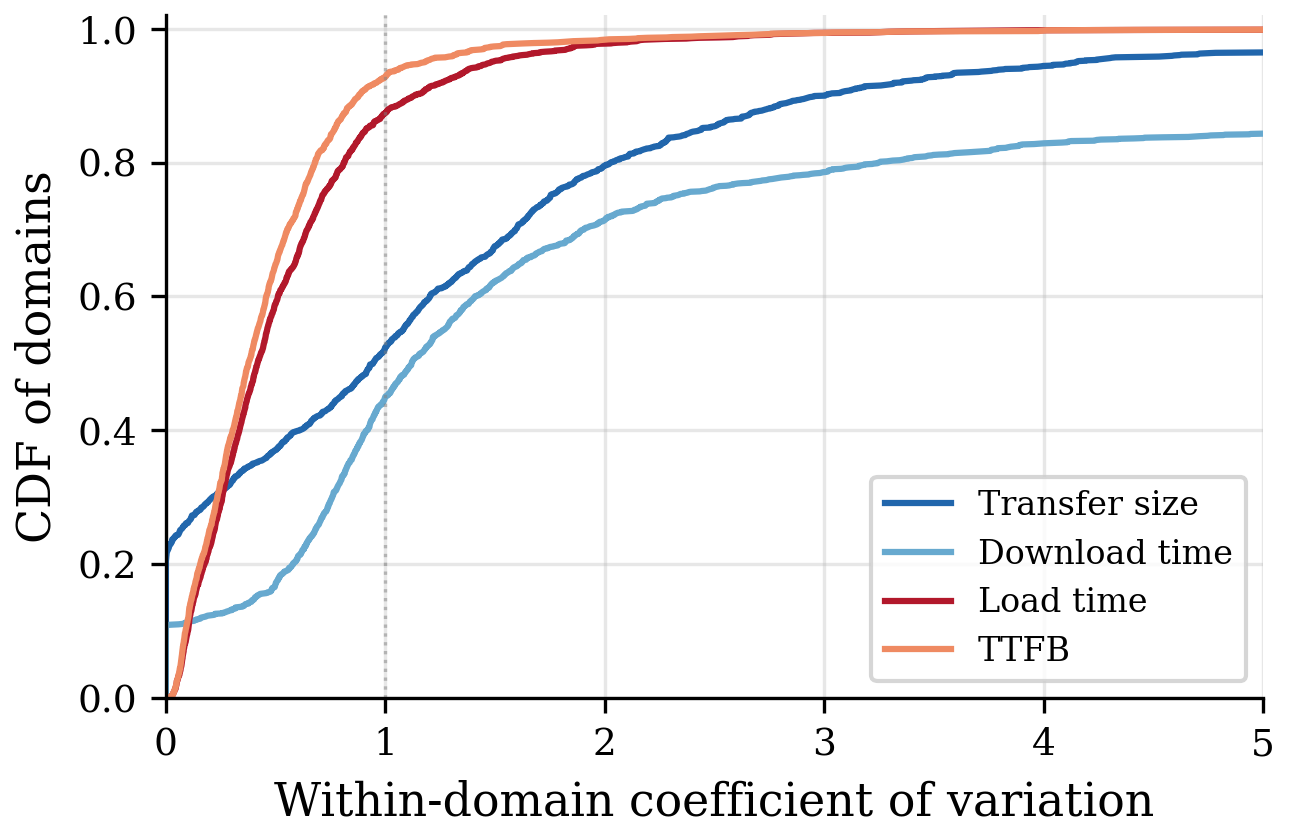
\includegraphics[width=0.85\columnwidth]{figures/fig7_within_domain_cv.pdf}
    \caption{CDF of within-domain coefficient of variation by target. Transfer size and download time have high intra-domain variance (URL-predictable); TTFB and load time have low variance (network-dominated).}
    \label{fig:cv}
\end{figure}

% ============================================================
\section{Data}
\label{sec:data}
% ============================================================

\subsection{Source and Sampling}

We use the HTTP Archive June 2024 mobile crawl, filtering to third-party tracker requests in five categories (advertising, analytics, social, tag-manager, and consent-provider) as classified by HTTP Archive's third-party entity table.
The full dataset contains approximately 348 million tracker requests across 5,186 domains.

A 1\% deterministic sample is drawn via hash-based sampling:
\[
\texttt{MOD(ABS(FARM\_FINGERPRINT(page} \| \texttt{url)),~100) = 0}
\]
yielding \numrequests requests across \numdomains domains.
Hash-based sampling ensures reproducibility and uniform coverage across page--request combinations.

\subsection{Features}
\label{sec:features}

Features are organized by what Firefox observes at block time (Table~\ref{tab:features}).

\begin{table}[t]
\centering
\small
\begin{tabular}{llr}
\toprule
Group & Features & Dim. \\
\midrule
Domain identity & Target-encoded median, median by type & 2 \\
URL structure & Path depth, URL length, \#query params, extension & 12 \\
URL content & TF-IDF + SVD embedding of URL path & 50 \\
Request metadata & Resource type, initiator type, HTTP method & 10 \\
URL patterns & Regex flags (js, collect, image, sync, ad, api) & 6 \\
\midrule
\textbf{Total} & & \textbf{80} \\
\bottomrule
\end{tabular}
\caption{Feature groups. URL structure includes one-hot encoded file extension (8 categories). Request metadata includes one-hot encoded resource type (6), initiator type (3), and POST indicator.}
\label{tab:features}
\end{table}

\paragraph{Domain target encoding.}
The tracker domain (\numdomains unique values) is encoded as two statistics computed from the training split: median \texttt{transfer\_bytes} per domain, and median per (domain, resource type).
Unseen domains receive the global median.
This encoding is the single most important feature (Section~\ref{sec:feature-importance}).

\paragraph{TF-IDF URL embeddings.}
We tokenize each URL path by splitting on delimiters (\texttt{/ ? \& = . - \_}) and camelCase boundaries, lowercased, filtering to tokens $\geq 2$ characters.
TF-IDF vectors are computed with sublinear TF ($\log(1+\text{tf})$), unigram and bigram features, vocabulary capped at 50K terms, minimum document frequency 5.
Truncated SVD reduces the sparse matrix to 50 dense dimensions, explaining 54.5\% of variance.

The leading SVD components are semantically interpretable:
component 1 separates \texttt{/collect} endpoints (beacons) from all others;
component 2 captures \texttt{/gtag/js} and \texttt{analytics.js} (script bundles);
components 3--5 distinguish tracking pixels, ad-server paths, and cookie synchronization endpoints.
These correspond to the distinctions that hand-crafted regex features target, but are discovered automatically.

\paragraph{Regex URL features.}
Six binary features flag URL path patterns: JavaScript (\texttt{\.js|sdk|gtm}), collection endpoints (\texttt{collect|beacon|pixel}), images (\texttt{\.gif|\.png|1x1}), sync (\texttt{sync|match|cookie}), ads (\texttt{/ad/|pagead|prebid}), and APIs (\texttt{/api/|/v[0-9]/}).
These are included alongside TF-IDF embeddings; Section~\ref{sec:feature-ablation} ablates both.

\subsection{Target Distribution}

The primary target is \texttt{transfer\_bytes}: on-wire response size in bytes.
Its distribution is severely zero-inflated (39.5\% exact zeros, mostly tracking beacons) with a heavy right tail (max 8.6\,MB, mean 13,607, median 43), as shown in Figure~\ref{fig:target-dist}.
This bimodal structure---a spike at zero and a long right tail---motivates the Tweedie loss (Section~\ref{sec:methods}).
We also evaluate timing targets; see Section~\ref{sec:multi-target}.

\begin{figure}[t]
    \centering
    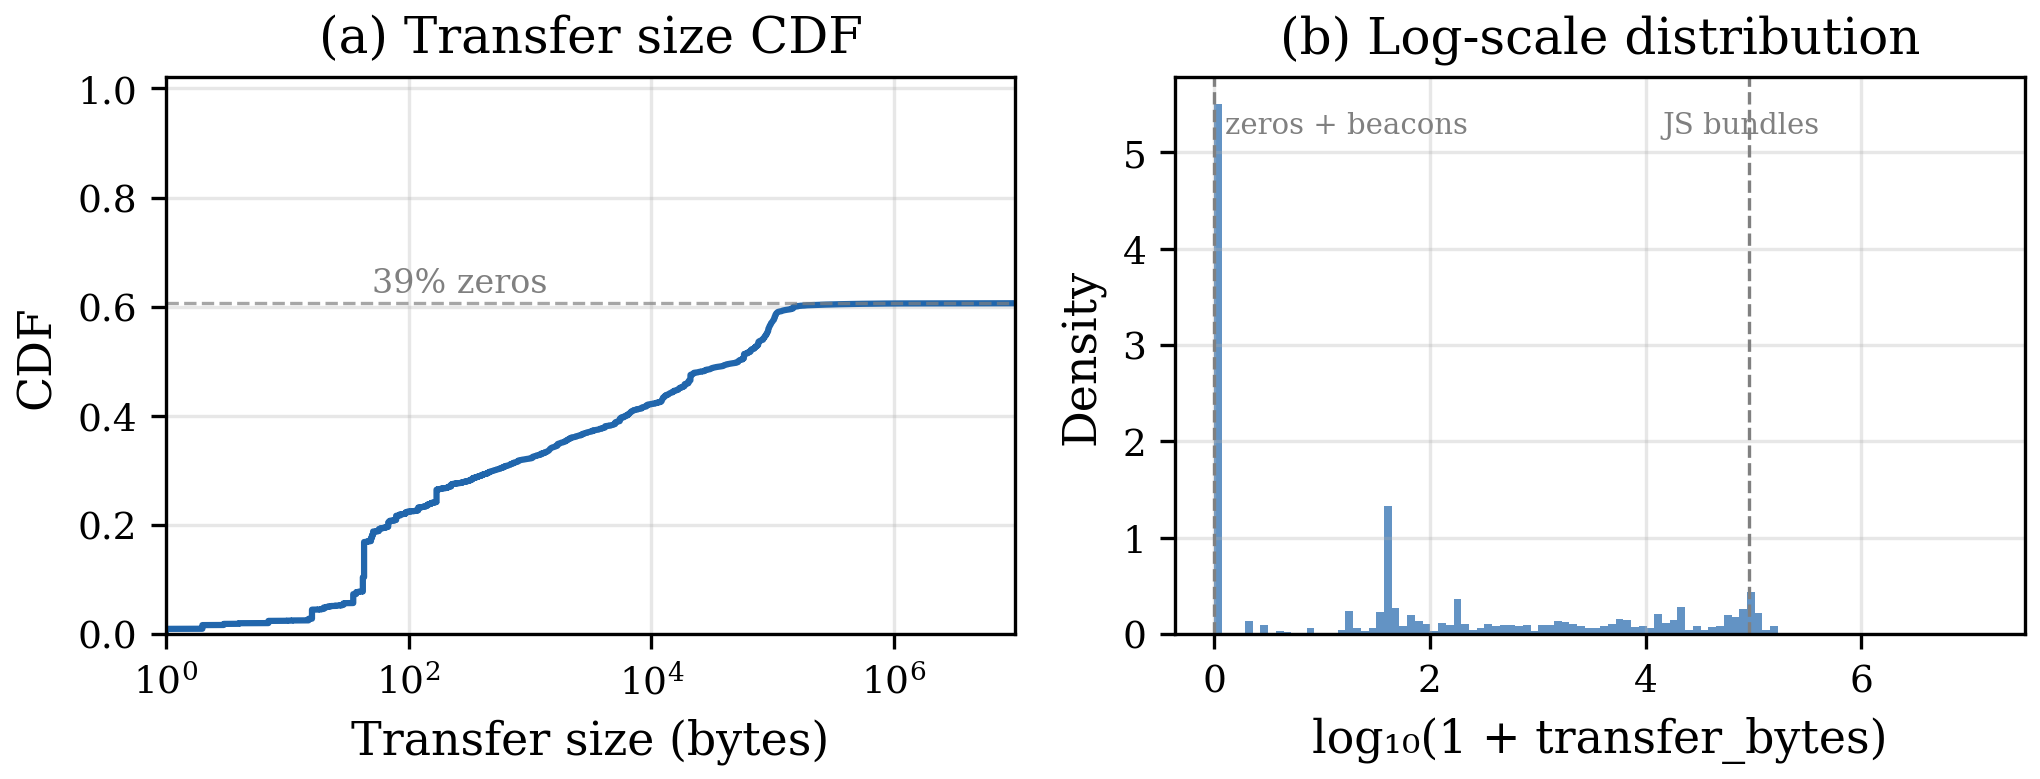
\includegraphics[width=\columnwidth]{figures/fig1_target_distribution.pdf}
    \caption{Transfer size distribution. (a)~CDF showing that 39\% of requests have zero transfer size (beacons) and the distribution spans five orders of magnitude. (b)~Log-scale histogram revealing the bimodal structure: a spike at zero/near-zero and a secondary mode around 90\,KB (JavaScript bundles).}
    \label{fig:target-dist}
\end{figure}

\subsection{Data Split}

Rows are split randomly: 70\% training (\numtrainrows), 15\% validation (523,624), 15\% test (\numtestrows).
Row-level splitting is appropriate because Firefox will have HTTP Archive statistics for all Disconnect-list domains at deployment; domain identity is a known feature at inference time.
Target encodings are computed exclusively from the training split.

% ============================================================
\section{Methods}
\label{sec:methods}
% ============================================================

\subsection{Baselines}
\label{sec:baselines-method}

We evaluate four lookup table baselines of increasing granularity, each using the training-set median as the predicted value:
(1)~global median;
(2)~per-domain median with global fallback;
(3)~per-(domain, resource type) median with domain then global fallback;
(4)~per-(domain, URL path) median with (domain, type), domain, then global fallback.

\subsection{XGBoost with Tweedie Loss}

The zero-inflated, heavy-tailed transfer size distribution motivates the Tweedie loss~\cite{jorgensen1987exponential} with variance power $p \in (1,2)$:
\[
\ell_\text{Tweedie}(\hat{y}, y) = -y \frac{\hat{y}^{1-p}}{1-p} + \frac{\hat{y}^{2-p}}{2-p}
\]
This penalizes errors proportionally to predicted magnitude, focusing capacity on high-cost requests rather than the mass of near-zero beacons.
We tune $p$ via ablation (Section~\ref{sec:loss-ablation}).

All XGBoost models use 500 trees, max depth 8, learning rate 0.05, row subsampling 0.8, column subsampling 0.7, minimum child weight 10, with early stopping (patience 20) on the validation set.
An offset of $+1$ is applied to targets before training (reversed after prediction) to satisfy the Tweedie constraint $\hat{y} > 0$.

% ============================================================
\section{Results}
\label{sec:results}
% ============================================================

\subsection{Baseline Comparison}
\label{sec:baselines}

Table~\ref{tab:main-results} presents the main result: a hierarchy of approaches with bootstrap 95\% confidence intervals.

\begin{table}[t]
\centering
\small
\begin{tabular}{lrrl}
\toprule
Approach & MAE & 95\% CI & Spearman $\rho$ \\
\midrule
Global median & 13,661 & --- & --- \\
Domain LUT & 7,878 & --- & --- \\
Domain+type LUT & 6,597 & [6,426, 6,790] & 0.926 \\
Path LUT (with fallback) & 3,797 & [3,623, 3,984] & 0.934 \\
\textbf{XGBoost Tweedie} & \textbf{3,466} & \textbf{[3,314, 3,627]} & \textbf{0.945} \\
\bottomrule
\end{tabular}
\caption{Transfer size prediction on the test set (\numtestrows requests). MAE in bytes. Bootstrap CIs from 1,000 resamples. The model's CI does not overlap with the path LUT's.}
\label{tab:main-results}
\end{table}

The XGBoost model with Tweedie loss achieves the lowest MAE (3,466 bytes), reducing error by 47.5\% relative to the domain+type LUT and by 8.7\% relative to the path LUT (Figure~\ref{fig:baseline-ladder}).
Notably, the model's confidence interval [3,314, 3,627] does not overlap with the path LUT's [3,623, 3,984], confirming the improvement is statistically significant.

\begin{figure}[t]
    \centering
    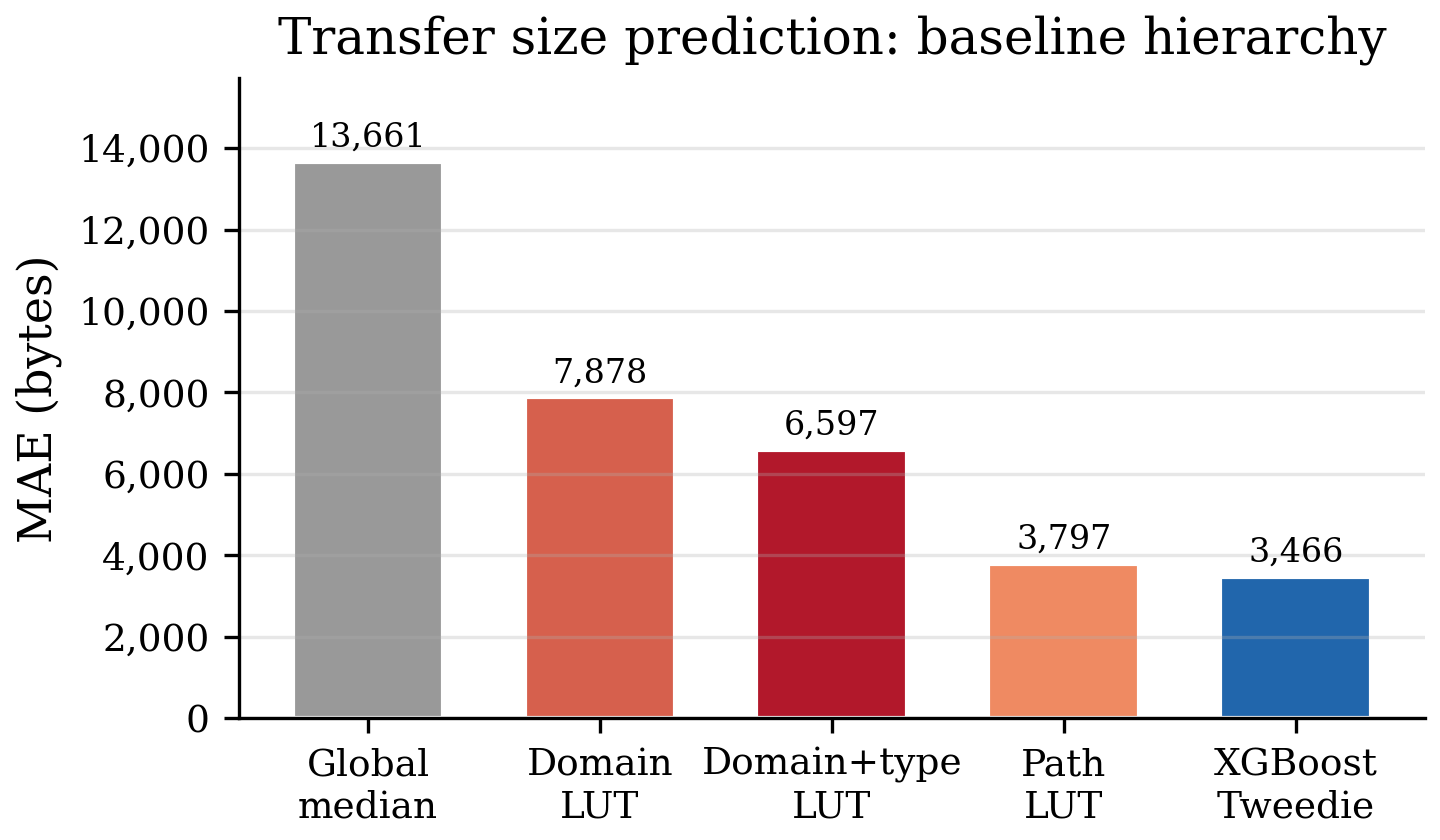
\includegraphics[width=\columnwidth]{figures/fig2_baseline_ladder.pdf}
    \caption{Transfer size MAE across the baseline hierarchy. Each step adds information: domain identity, resource type, URL path, and finally learned features via the model.}
    \label{fig:baseline-ladder}
\end{figure}

\paragraph{The model outperforms exact-path lookup.}
Decomposing by path coverage reveals a surprising result (Table~\ref{tab:decomposition}, Figure~\ref{fig:path-decomp}).
On the 91.6\% of test rows where the path LUT has an exact training match, the model still achieves lower MAE (1,346 vs.\ 1,448).
The model regularizes across similar URL structures: a path appearing 3 times in training has a noisy median, while the model smooths predictions using domain statistics, URL length, and TF-IDF embeddings.
On the 8.4\% of rows with unseen paths---which are disproportionately expensive (mean 35,876 bytes)---both approaches struggle, but the model's error (26,655) is lower than the path LUT's domain+type fallback (29,491).

\begin{figure}[t]
    \centering
    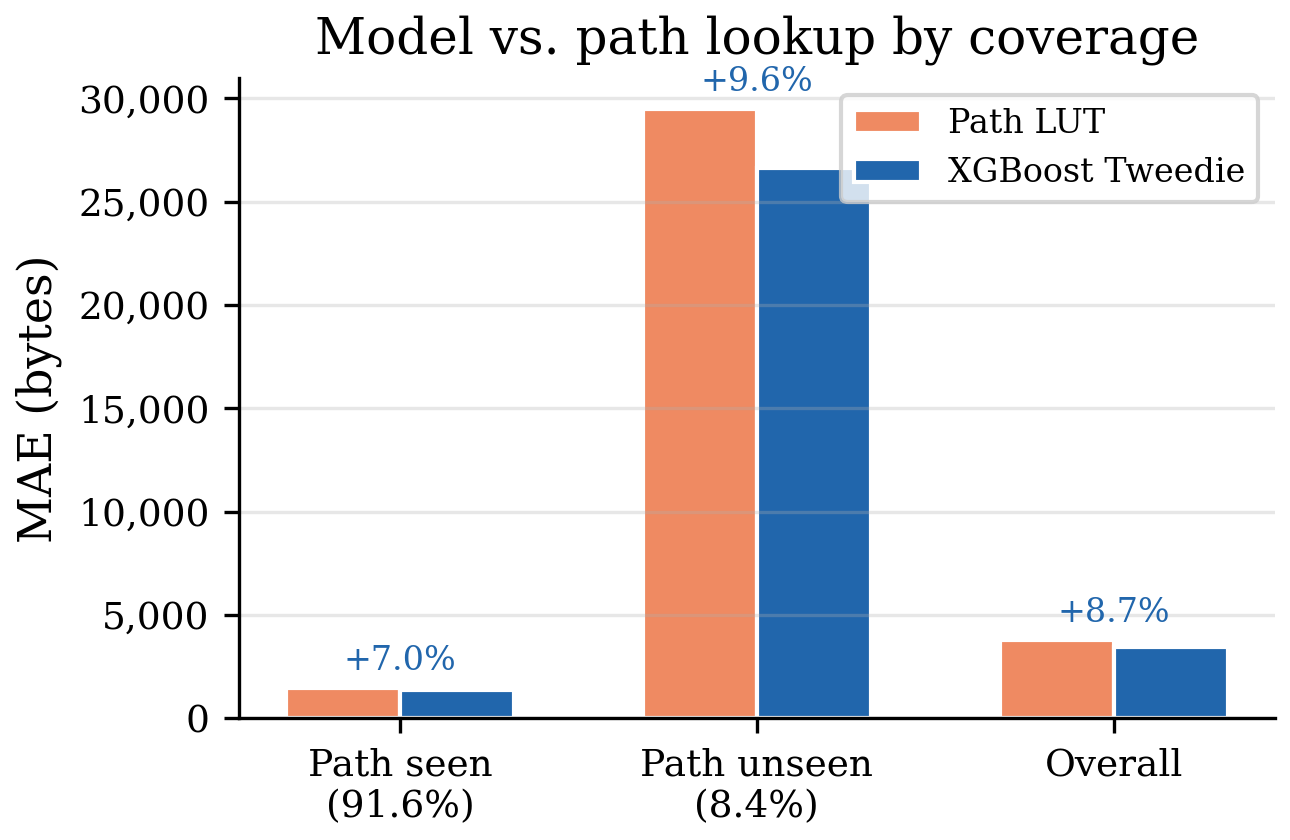
\includegraphics[width=0.9\columnwidth]{figures/fig9_path_decomposition.pdf}
    \caption{The model outperforms the path LUT on both seen paths (regularization beats noisy memorization) and unseen paths (generalization beats fallback).}
    \label{fig:path-decomp}
\end{figure}

\begin{table}[t]
\centering
\small
\begin{tabular}{lrrr}
\toprule
Subset & $n$ & Path LUT MAE & Model MAE \\
\midrule
Path seen in training (91.6\%) & 479,775 & 1,448 & \textbf{1,346} \\
Path unseen (8.4\%) & 43,849 & 29,491 & \textbf{26,655} \\
\midrule
Overall & 523,624 & 3,797 & \textbf{3,466} \\
\bottomrule
\end{tabular}
\caption{Model vs.\ path LUT decomposed by path coverage. The model outperforms the LUT on \emph{both} subsets.}
\label{tab:decomposition}
\end{table}

\subsection{Loss Function Ablation}
\label{sec:loss-ablation}

To isolate the effect of loss function from architecture, we train XGBoost with five loss configurations on identical data and features (Table~\ref{tab:loss-ablation}).

\begin{table}[t]
\centering
\small
\begin{tabular}{lrrr}
\toprule
Loss function & MAE & vs.\ LUT & Spearman $\rho$ \\
\midrule
Squared error & 4,527 & +31.4\% & 0.738 \\
Tweedie ($p = 1.2$) & 3,486 & +47.2\% & 0.937 \\
\textbf{Tweedie ($p = 1.5$)} & \textbf{3,466} & \textbf{+47.5\%} & \textbf{0.945} \\
Tweedie ($p = 1.8$) & 3,597 & +45.5\% & 0.949 \\
\bottomrule
\end{tabular}
\caption{Loss function comparison for transfer size. Architecture (XGBoost, 500 trees) and features (80 dimensions) are held constant. ``vs.\ LUT'' is improvement over domain+type LUT (MAE 6,597). Huber loss ($\delta=10{,}000$) diverged (MAE 19,373) and is omitted.}
\label{tab:loss-ablation}
\end{table}

Tweedie loss at $p=1.5$ achieves the best MAE (3,466), outperforming squared error by 23\% (3,466 vs.\ 4,527) on identical features (Figure~\ref{fig:loss-ablation}).
The Tweedie power parameter is relatively robust: $p \in [1.2, 1.8]$ all outperform squared error by at least 17\%.
The mechanism is that squared error allocates model capacity uniformly across the prediction range, spending most effort on the 39.5\% of near-zero beacons where any small prediction suffices, while Tweedie loss weights errors by predicted magnitude and focuses on the high-cost tail that dominates aggregate accuracy.

\begin{figure}[t]
    \centering
    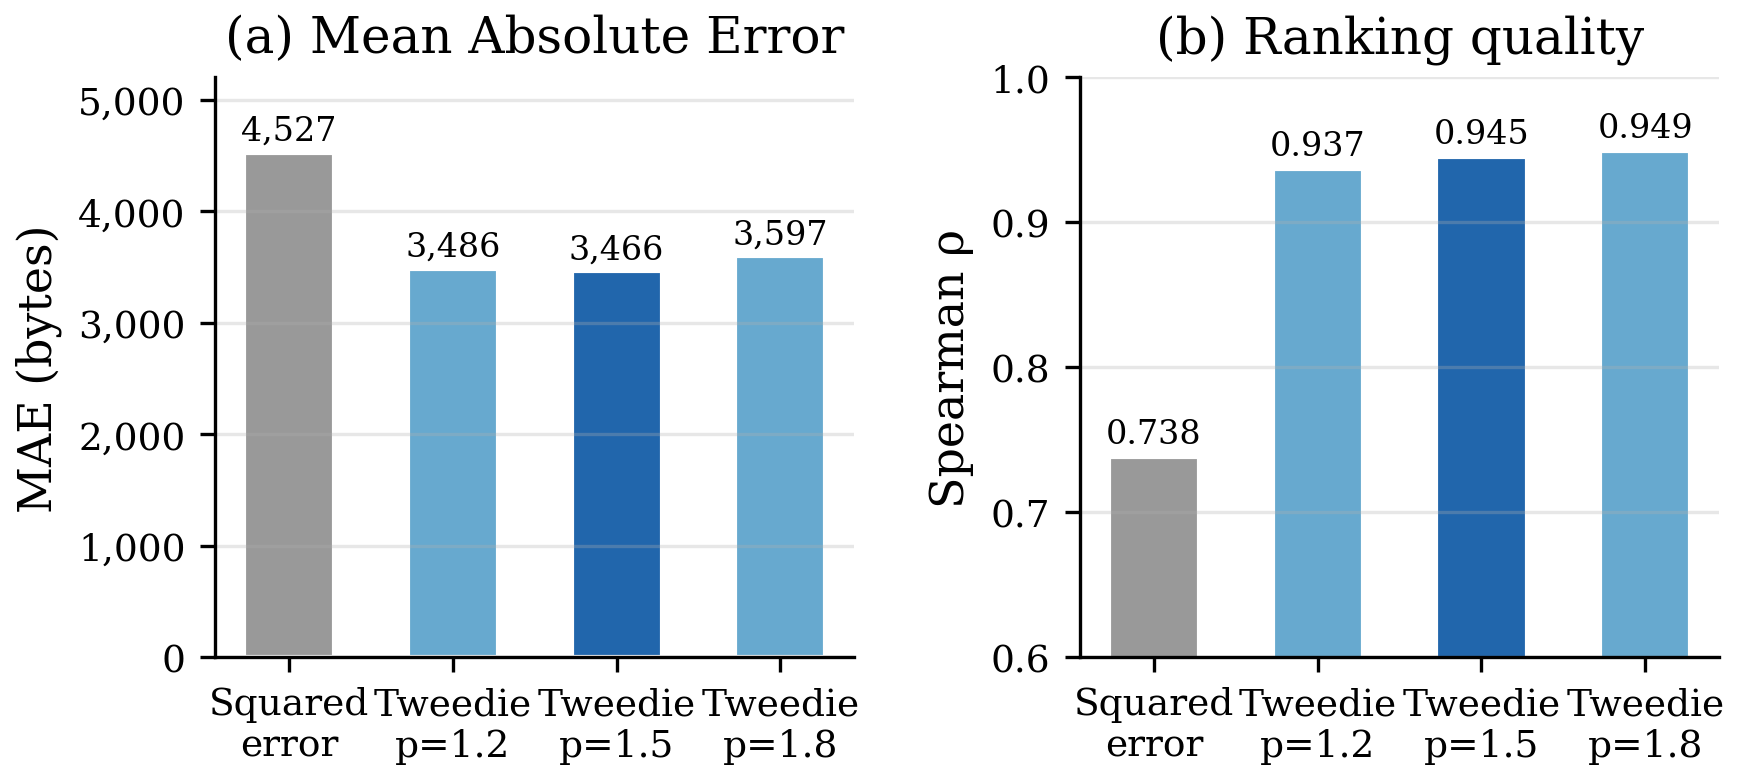
\includegraphics[width=\columnwidth]{figures/fig5_loss_ablation.pdf}
    \caption{Loss function ablation. (a)~Tweedie loss reduces MAE by 23\% over squared error. (b)~The Spearman ranking quality gap is even larger (0.945 vs.\ 0.738).}
    \label{fig:loss-ablation}
\end{figure}

\subsection{Feature Ablation}
\label{sec:feature-ablation}

Table~\ref{tab:feature-ablation} ablates the two URL content feature groups: hand-crafted regex flags and TF-IDF embeddings.

\begin{table}[t]
\centering
\small
\begin{tabular}{lrr}
\toprule
URL content features & MAE & vs.\ regex only \\
\midrule
Regex only (6 binary features) & 4,251 & --- \\
TF-IDF only (50 SVD dimensions) & 3,548 & +16.5\% \\
\textbf{Both (56 features)} & \textbf{3,466} & \textbf{+18.5\%} \\
\bottomrule
\end{tabular}
\caption{Feature ablation for URL content representation. All models use Tweedie loss and include domain, URL structure, and request metadata features. TF-IDF embeddings provide a larger improvement (16.5\%) than adding regex features on top of them (2.0\%).}
\label{tab:feature-ablation}
\end{table}

TF-IDF embeddings alone (MAE 3,548) nearly match the full feature set (3,466) and substantially outperform regex features alone (4,251), as shown in Figure~\ref{fig:feat-ablation}.
Adding regex features on top of TF-IDF provides only a marginal 2.3\% further improvement, suggesting the embeddings subsume most of the signal in the hand-crafted patterns.
This is expected: the TF-IDF vocabulary captures \texttt{collect}, \texttt{pixel}, \texttt{sdk}, \texttt{sync}, and other patterns that the regex features target, while also discovering patterns the researcher did not anticipate (e.g., Privacy Sandbox \texttt{register-trigger} paths).

\begin{figure}[t]
    \centering
    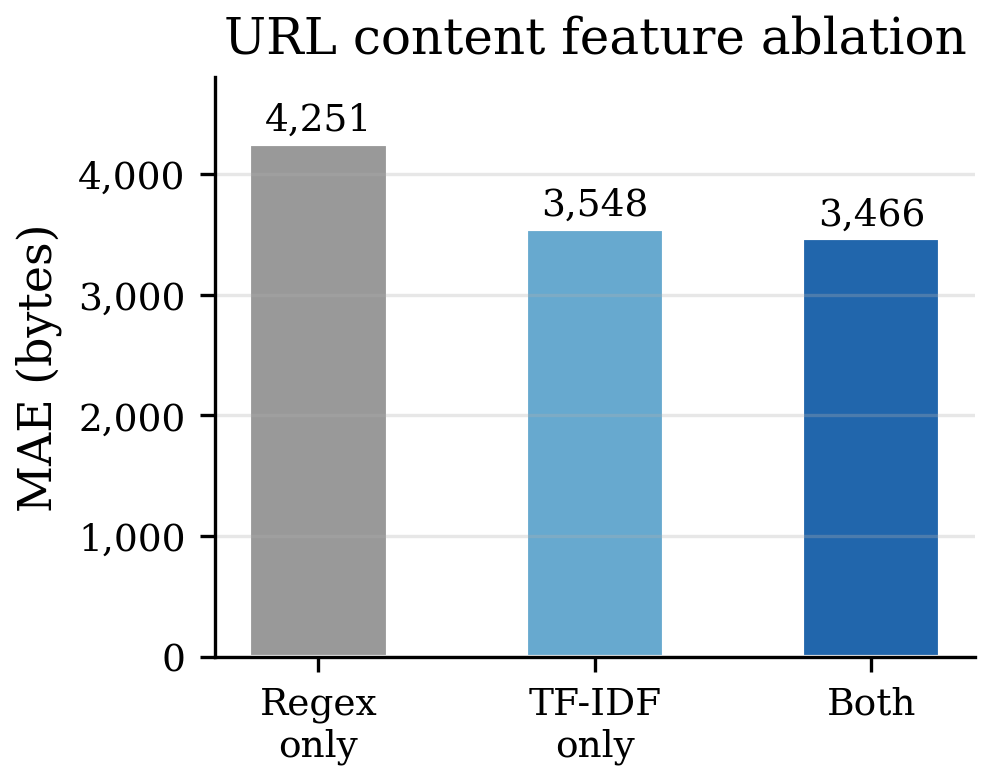
\includegraphics[width=0.65\columnwidth]{figures/fig8_feature_ablation.pdf}
    \caption{URL content feature ablation. TF-IDF embeddings alone nearly match the full model; hand-crafted regex features add little on top.}
    \label{fig:feat-ablation}
\end{figure}

\subsection{Feature Importance}
\label{sec:feature-importance}

XGBoost feature importance (gain-based) reveals that the target-encoded domain+type median dominates (8.65\% of total gain), followed by resource type indicators (\texttt{rt\_other}: 5.87\%, \texttt{rt\_text}: 3.09\%), URL pattern flags (\texttt{path\_has\_sync}: 4.88\%), and file extension indicators (\texttt{ext\_html}: 4.08\%).
TF-IDF embedding dimensions contribute collectively: 8 of the top 15 features are embedding dimensions, individually accounting for 1.4--3.2\% of gain each.
No single embedding dimension dominates, consistent with the distributed URL representation learned by SVD.

\subsection{Results by Resource Type}
\label{sec:by-type}

\begin{table}[t]
\centering
\small
\begin{tabular}{lrrrr}
\toprule
Resource type & $n$ & LUT MAE & Model MAE & Improv. \\
\midrule
Script & 144,676 & 12,996 & 3,135 & \textbf{+75.9\%} \\
CSS & 6,142 & 6,222 & 2,084 & +66.5\% \\
HTML & 92,438 & 2,246 & 1,294 & +42.4\% \\
Image & 136,698 & 8,330 & 7,428 & +10.8\% \\
Other (beacon) & 98,617 & 16 & 16 & +4.6\% \\
Text & 42,984 & 292 & 303 & $-$3.8\% \\
\bottomrule
\end{tabular}
\caption{Transfer size MAE by resource type. Improvement is concentrated on script (+75.9\%) and CSS (+66.5\%) resources, which have both high variance and URL-discriminative structure.}
\label{tab:by-type}
\end{table}

The model's improvement is concentrated on resource types with high within-type variance and URL-discriminative structure (Table~\ref{tab:by-type}, Figure~\ref{fig:by-type}).
Scripts see a 75.9\% MAE reduction: the model distinguishes \texttt{/gtag/js} (93\,KB bundles) from \texttt{/collect} (0-byte beacons) served by the same domain.
For low-variance types (``other,'' mostly beacons; ``text''), the LUT's constant prediction is near-optimal and the model provides no benefit.

\begin{figure}[t]
    \centering
    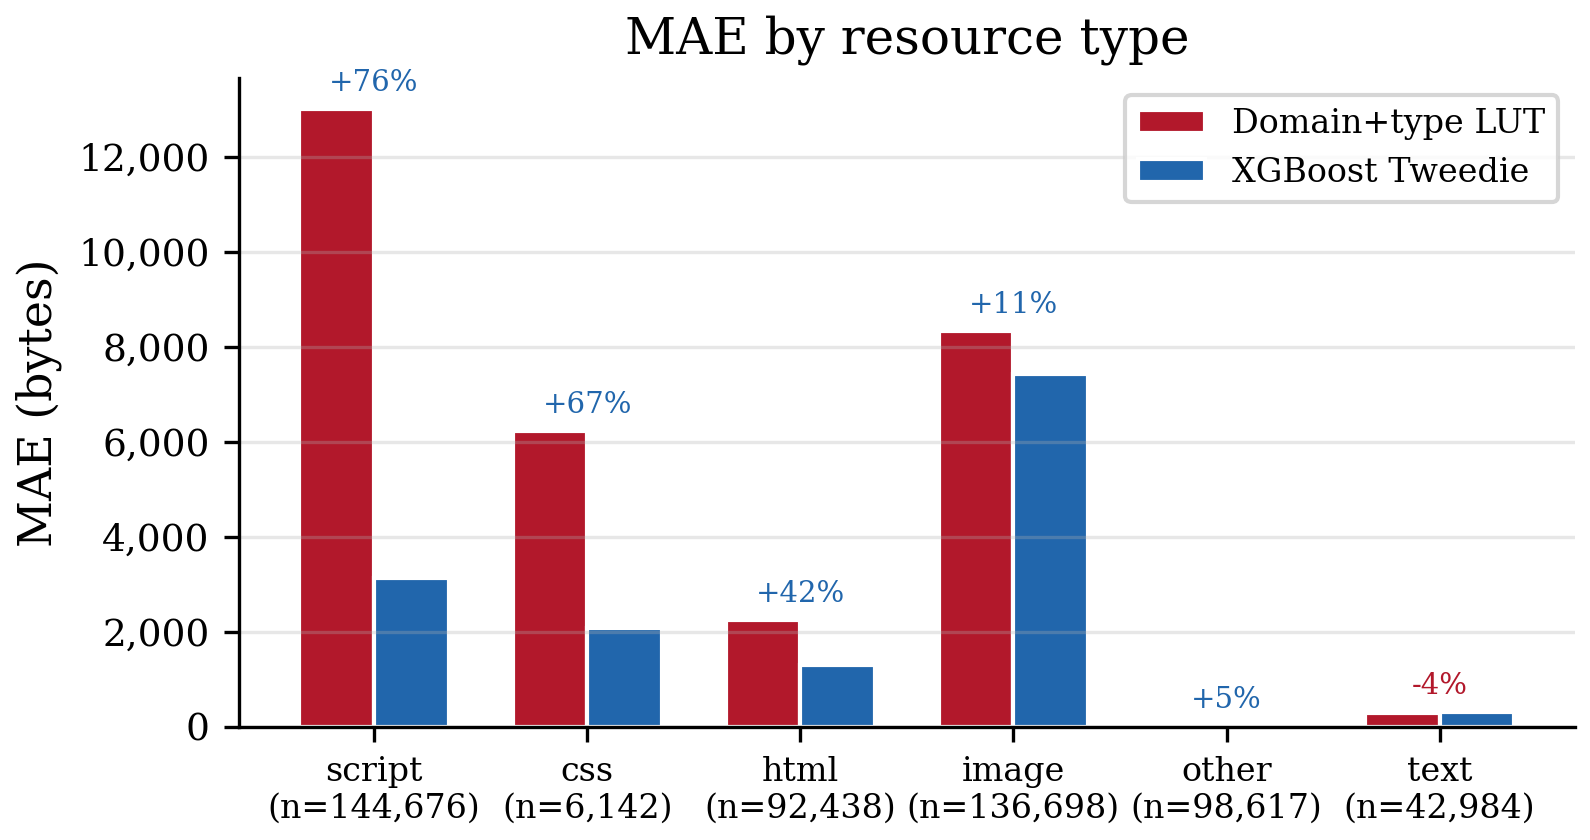
\includegraphics[width=\columnwidth]{figures/fig4_per_resource_type.pdf}
    \caption{MAE by resource type. The model's advantage is concentrated on scripts (+76\%) and CSS (+67\%), which have both high variance and URL-discriminative structure.}
    \label{fig:by-type}
\end{figure}

\subsection{Aggregation Accuracy}
\label{sec:aggregation}

Users see a weekly aggregate, not individual predictions.
We simulate weekly browsing by sampling $N$ blocked requests (with replacement, 2,000 trials), summing predicted and true transfer sizes, and computing percentage error.

\begin{table}[t]
\centering
\small
\begin{tabular}{lrrrr}
\toprule
& \multicolumn{2}{c}{Median \% error} & \multicolumn{2}{c}{Within 10\% of truth} \\
\cmidrule(lr){2-3} \cmidrule(lr){4-5}
$N$ (req/week) & Model & LUT & Model & LUT \\
\midrule
50 & 6.8\% & 20.8\% & 63.4\% & 25.2\% \\
100 & 6.3\% & 20.9\% & 65.6\% & 22.1\% \\
200 & 6.0\% & 21.9\% & 67.2\% & 13.6\% \\
500 & 5.1\% & 23.2\% & 75.5\% & 4.2\% \\
\bottomrule
\end{tabular}
\caption{Weekly aggregation accuracy for transfer size. The LUT's systematic bias compounds with more requests; the model's approximately symmetric errors cancel.}
\label{tab:aggregation}
\end{table}

At 200 blocked requests per week (a typical browsing load), the model's weekly total has 6.0\% median error and falls within 10\% of truth 67.2\% of the time (Table~\ref{tab:aggregation}).
The LUT's error is 21.9\%, and only 13.6\% of weeks are within 10\%.

The gap \emph{widens} with more requests (Figure~\ref{fig:agg-cdf}): at $N=500$, the model improves to 5.0\% median error while the LUT degrades to 23.0\%.
This occurs because the LUT has a systematic directional bias for certain URL patterns (e.g., consistently overpredicting beacons and underpredicting scripts), which compounds in summation.
The model's errors are approximately mean-zero and cancel via the law of large numbers.

\begin{figure}[t]
    \centering
    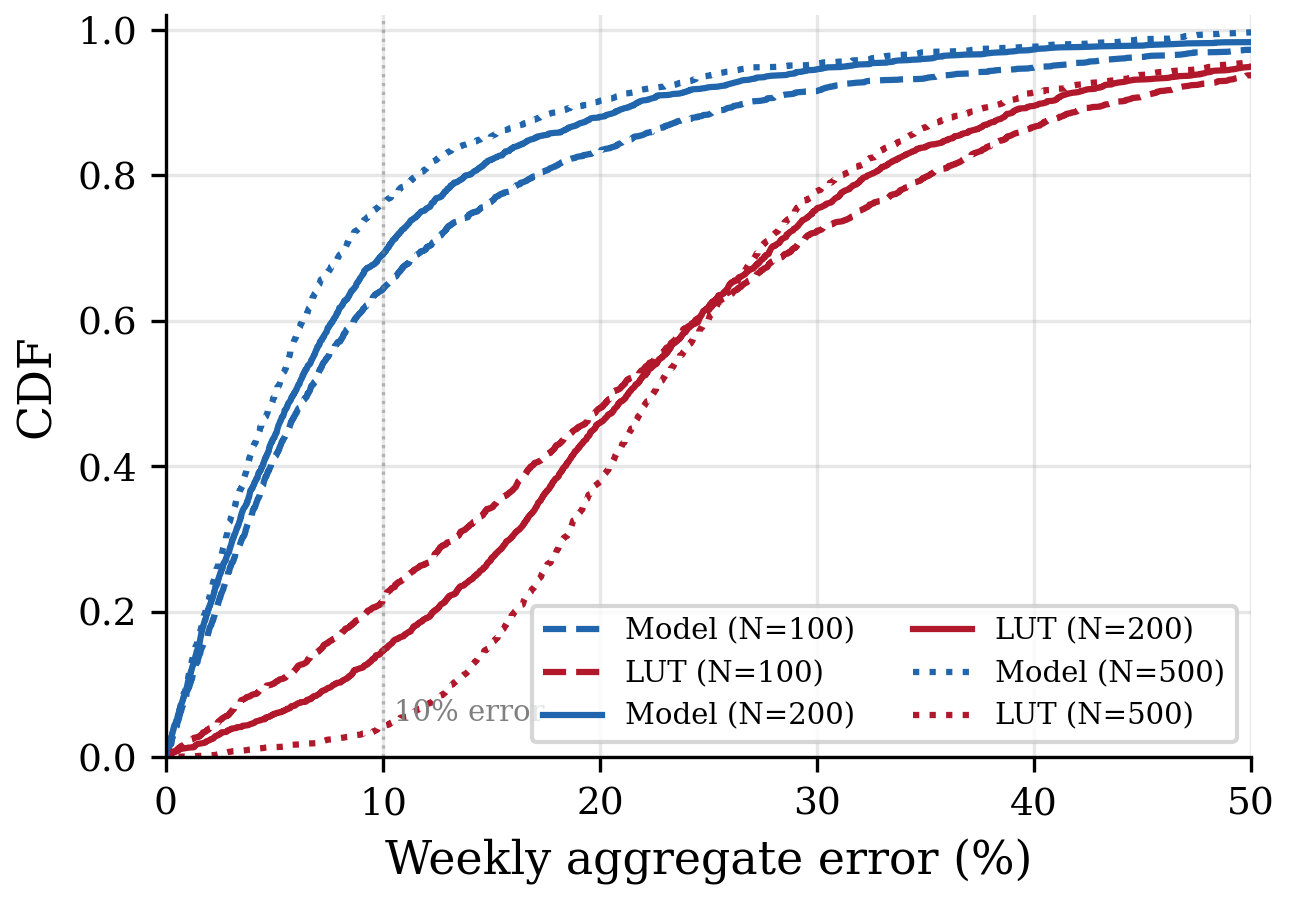
\includegraphics[width=\columnwidth]{figures/fig3_aggregation_cdf.pdf}
    \caption{CDF of weekly aggregation error. The model (blue) concentrates mass near zero, while the LUT (red) has a long tail of high-error weeks. The gap widens with more requests as the LUT's systematic bias compounds.}
    \label{fig:agg-cdf}
\end{figure}

\paragraph{Robustness to correlated browsing.}
The uniform simulation assumes i.i.d.\ request sampling, but real browsing is correlated: users visit the same 10--20 sites repeatedly.
Since domain target encoding is the model's top feature, within-domain errors may be correlated and cancel less effectively.
We test this by sampling 15 domains per trial (with replacement), then drawing $N$ requests from those domains only.

\begin{table}[t]
\centering
\small
\begin{tabular}{lrrrr}
\toprule
& \multicolumn{2}{c}{Uniform} & \multicolumn{2}{c}{Domain-correlated} \\
\cmidrule(lr){2-3} \cmidrule(lr){4-5}
$N$ & Model & LUT & Model & LUT \\
\midrule
50 & 7.1\% & 21.0\% & 14.2\% & 34.5\% \\
100 & 6.7\% & 21.1\% & 12.5\% & 34.2\% \\
200 & 6.3\% & 22.2\% & 12.9\% & 36.4\% \\
500 & 5.0\% & 23.0\% & 11.2\% & 36.7\% \\
\bottomrule
\end{tabular}
\caption{Aggregation accuracy under uniform vs.\ domain-correlated browsing (median \% error). Correlated browsing roughly doubles the model's error (6.3\% $\to$ 12.9\% at $N\!=\!200$) but nearly triples the LUT's (22.2\% $\to$ 36.4\%). The model's relative advantage \emph{increases} under correlation.}
\label{tab:correlated}
\end{table}

Correlated browsing approximately doubles the model's median error at $N=200$ (6.3\% $\to$ 12.9\%), confirming the reviewer intuition that within-domain error correlation reduces cancellation.
However, the LUT's error increases even more (22.2\% $\to$ 36.4\%), because its systematic per-domain bias is amplified when browsing concentrates on fewer domains.
The model's relative advantage actually \emph{increases} under correlated browsing: the model is $2.8\times$ better than the LUT under domain-correlated sampling versus $3.5\times$ under uniform sampling (Table~\ref{tab:correlated}).

\subsection{Multi-Target Results}
\label{sec:multi-target}

Beyond transfer size, we evaluate three timing targets using the same features and Tweedie loss.

\begin{table}[t]
\centering
\small
\begin{tabular}{lrrrl}
\toprule
Target & LUT MAE & XGB MAE & Improv. & Agg.\ err (200) \\
\midrule
\texttt{transfer\_bytes} & 6,597 & \textbf{3,466} & +47.5\% & 6.0\% \\
\texttt{download\_ms} & 73 & \textbf{56} & +23.7\% & 16.6\% \\
\texttt{load\_ms} & 117 & 121 & $-$3.1\% & 5.6\% \\
\texttt{ttfb\_ms} & 67 & 76 & $-$12.7\% & 4.0\% \\
\bottomrule
\end{tabular}
\caption{Multi-target results. Per-request MAE improvement is strong for transfer size and download duration (both URL-dependent) but absent for latency metrics (network-dependent). However, aggregation error (rightmost column) favors the model on all targets.}
\label{tab:multi-target}
\end{table}

Per-request MAE tells two distinct stories (Table~\ref{tab:multi-target}).
Transfer size (+47.5\%) and download duration (+23.7\%) improve substantially---both are \emph{content-dependent} metrics where the URL determines the response size and hence the download time.
TTFB ($-$12.7\%) and total load time ($-$3.1\%) do not improve---these are \emph{network-dependent} metrics determined by server latency, geographic routing, and connection conditions.
The within-domain CV confirms this: transfer size has CV 0.94 (high, URL-predictable variance) while TTFB has CV 0.38 (low, noise-dominated variance).

However, the aggregation column reveals that the model's weekly estimates outperform the LUT on \emph{all four targets}, including TTFB (4.0\% vs.\ LUT's 13.8\%) and load time (5.6\% vs.\ 14.2\%), as shown in Figure~\ref{fig:multi-agg}.
The model's per-request errors on timing targets are roughly symmetric and cancel in aggregation, while the LUT's systematic bias compounds.

\begin{figure}[t]
    \centering
    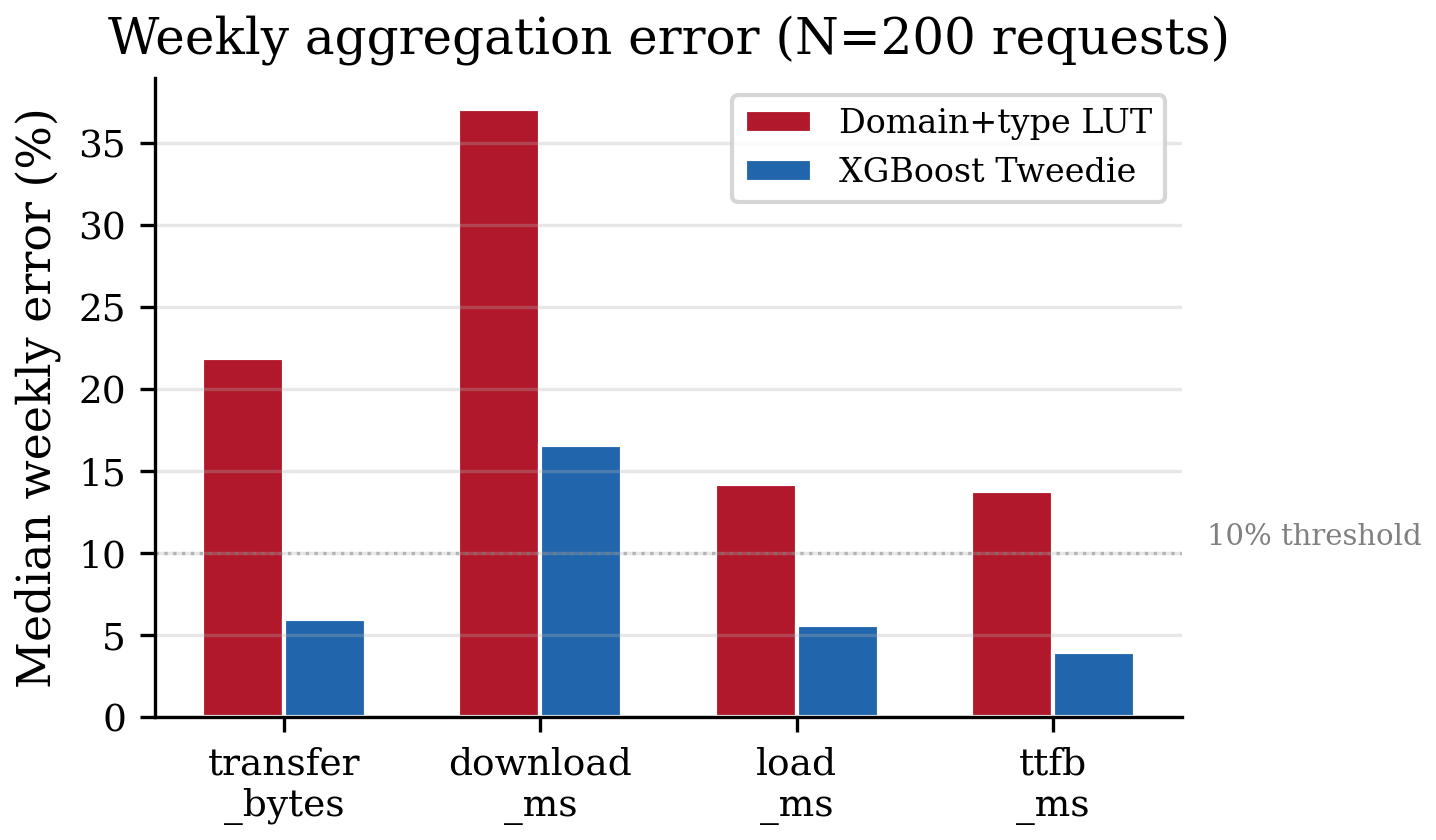
\includegraphics[width=\columnwidth]{figures/fig10_multi_target_agg.pdf}
    \caption{Weekly aggregation error across all four targets (N=200). The model outperforms the LUT on every target, including timing metrics where per-request MAE favored the LUT.}
    \label{fig:multi-agg}
\end{figure}

\subsection{Temporal Generalization}
\label{sec:temporal}

To evaluate whether the model generalizes across time, we train on June 2024 data and test on a held-out September 2024 crawl (3 months later, 3{,}137{,}748 requests).

\paragraph{Drift analysis.}
Of the 3,612 tracker domains in September, 88.2\% also appear in the June training set; 11.8\% are new.
URL path overlap is lower: only 14.9\% of unique September paths were seen in June training, though these cover 85.1\% of September \emph{rows} (frequent paths recur; rare paths are ephemeral).
The transfer size distribution is stable: June and September have identical medians (43 bytes) and similar means (13,621 vs.\ 14,258).

\paragraph{Results.}

\begin{table}[t]
\centering
\small
\begin{tabular}{lrrr}
\toprule
& June (in-dist) & Sep (temporal) & Degradation \\
\midrule
Domain+type LUT MAE & 6,597 & 6,723 & +1.9\% \\
Path LUT MAE & 3,797 & 4,966 & +30.8\% \\
\textbf{XGBoost Tweedie MAE} & \textbf{3,466} & \textbf{4,517} & \textbf{+30.3\%} \\
\quad 95\% CI & [3,314, 3,627] & [4,458, 4,581] & \\
\quad Spearman $\rho$ & 0.945 & 0.942 & \\
\quad vs.\ LUT & +47.5\% & +32.8\% & \\
\midrule
\multicolumn{3}{l}{\emph{Aggregation (N=200):}} \\
\quad Model med.\ err & 6.1\% & 10.1\% & \\
\quad LUT med.\ err & 21.8\% & 21.5\% & \\
\midrule
\multicolumn{3}{l}{\emph{Scripts only:}} \\
\quad Model MAE & 3,135 & 6,428 & \\
\quad LUT MAE & 12,996 & 13,021 & \\
\quad Improvement & +75.9\% & +50.6\% & \\
\bottomrule
\end{tabular}
\caption{Temporal generalization: train on June 2024, test on September 2024. The model degrades by 30\% but retains a 32.8\% advantage over the LUT. Ranking quality ($\rho$) is nearly unchanged. Path coverage drops from 91.6\% to 85.1\%.}
\label{tab:temporal}
\end{table}

The model's MAE degrades by 30.3\% (3,466 $\to$ 4,517) over three months (Table~\ref{tab:temporal}).
The path LUT degrades by a similar amount (30.8\%), while the domain+type LUT barely changes (+1.9\%)---its coarser granularity makes it more temporally stable but permanently less accurate.

Critically, the model retains a \textbf{32.8\% advantage over the LUT} on September data, compared to 47.5\% on June.
Ranking quality is nearly unchanged ($\rho = 0.942$ vs.\ 0.945).
The weekly aggregation estimate degrades from 6.1\% to 10.1\% median error---still substantially below the LUT's 21.5\%.
Scripts remain the strongest category, with the model achieving +50.6\% improvement in September versus +75.9\% in June.

The degradation is driven by URL path churn: only 14.9\% of unique September paths were seen in June, compared to the 91.6\% coverage within the June random split.
This suggests \textbf{quarterly retraining} on fresh HTTP Archive data to maintain accuracy, which is feasible given the monthly crawl cadence.

% ============================================================
\section{Analysis}
\label{sec:analysis}
% ============================================================

\subsection{Domain-Level Estimation Does Not Need ML}
\label{sec:domain-level}

A natural first approach is domain-level scoring: assign each tracker domain a static cost score using aggregated HTTP Archive features.
We built this pipeline for 4,592 domains, training XGBoost on 19 features to predict CPU and network cost scores (Spearman $\rho = 0.751$ and $0.999$ respectively).

The problem does not require machine learning.
Of the 4,592 domains, 2,185 (48\%) have direct Lighthouse CPU measurements and need no prediction.
The remaining 2,407 (52\%) fall below Lighthouse's $\sim$50\,ms reporting threshold and are uniformly inexpensive.
KS tests confirm the two populations are disjoint on every feature ($p < 0.001$; median \texttt{max\_script\_bytes}: 20,338 vs.\ 585).
Self-training~\cite{yarowsky1995unsupervised} produced zero improvement because the feature-space disjointness prevented any unlabeled domain from receiving a confident pseudo-label.

This negative result has a constructive implication: it establishes the criteria for a genuine prediction problem in this domain.
The domain-level formulation fails the test because labels are available (or trivially assignable) for both populations.
The per-request formulation passes: blocked requests have no response, and the URL-level variance (Section~\ref{sec:lut-motivation}) is too large for lookup tables to resolve.

\subsection{Why Tweedie Loss Outperforms Squared Error}

The transfer size distribution is zero-inflated: 39.5\% of values are exactly zero (beacons), while the remaining 60.5\% span five orders of magnitude.
Squared error treats a 100-byte error on a beacon identically to a 100-byte error on a 170\,KB script.
Tweedie loss with $p > 1$ scales the penalty by $\hat{y}^{2-p}$, effectively down-weighting near-zero predictions where absolute error is already small and up-weighting large predictions where accuracy matters for the aggregate.

This explains the 23\% MAE gap (3,466 vs.\ 4,527).
It also explains why the gap translates to an even larger aggregation advantage: the beacons that squared error over-optimizes for contribute negligibly to the weekly total, while the scripts that Tweedie prioritizes dominate it.
Figure~\ref{fig:pred-actual} confirms the model tracks the diagonal across five orders of magnitude, with tightest predictions in the 10\,KB--100\,KB range (JavaScript bundles).

\begin{figure}[t]
    \centering
    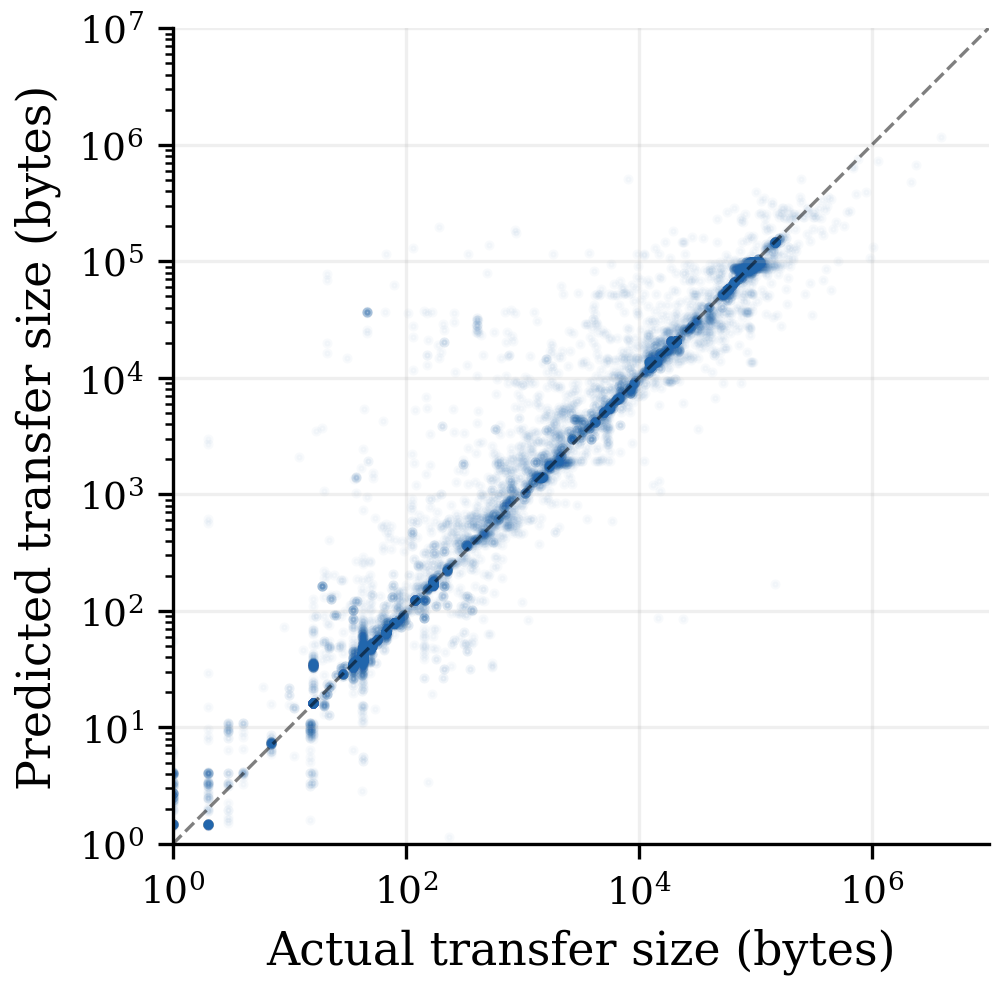
\includegraphics[width=0.75\columnwidth]{figures/fig6_pred_vs_actual.pdf}
    \caption{Predicted vs.\ actual transfer size (log scale, 20K random test samples). The model tracks the diagonal across five orders of magnitude.}
    \label{fig:pred-actual}
\end{figure}

% ============================================================
\section{Deployment Considerations}
\label{sec:deployment}
% ============================================================

\paragraph{Feature availability.}
When ETP intercepts a request, Firefox's \texttt{nsIChannel} and \texttt{nsILoadInfo} interfaces expose the request URI (maps to all URL features), content policy type (maps to resource type), loading principal (maps to initiator type), and HTTP method.
The TF-IDF vocabulary and SVD projection matrix are static artifacts ($\sim$2\,MB) shipped alongside the model.

\paragraph{Model format.}
The XGBoost model exports to ONNX format ($\sim$500\,KB for 500 trees).
Inference latency is on the order of microseconds.
Since cost estimates are used for background aggregation rather than real-time decisions, latency is not a constraint.

\paragraph{Deployment status.}
This model is scheduled for release in Firefox in May 2026 as part of a New Tab privacy widget, surfacing per-request cost estimates to approximately 250 million daily active users.
Model updates are delivered via Firefox Remote Settings, the same mechanism used for the Disconnect list.
Monthly retraining on fresh HTTP Archive crawl data tracks changes in tracker SDK versions and URL structures.

% ============================================================
\section{Limitations}
\label{sec:limitations}
% ============================================================

\paragraph{Temporal stability.}
The model degrades by 30\% over three months (June $\to$ September 2024; Section~\ref{sec:temporal}), driven by URL path churn (only 14.9\% of unique September paths were seen in June).
The model retains a 32.8\% advantage over the LUT on September data, but quarterly retraining on fresh HTTP Archive crawls is recommended for deployment.
Longer-term degradation (6--12 months) has not been measured.

\paragraph{Timing metric validity.}
Transfer size is server-determined and browser-independent.
Timing metrics depend on network stack, hardware, and conditions.
HTTP Archive uses a fixed test environment (Moto G4, cable connection), so timing predictions are standardized-condition estimates rather than personalized predictions.
We report timing results but recommend deploying only the transfer size model.

\paragraph{Training--deployment population shift.}
The model trains on HTTP Archive's third-party entity list and deploys on Firefox's Disconnect list.
These overlap substantially but not completely.
Disconnect-only domains absent from HTTP Archive receive the global median fallback.

\paragraph{Server-side variation.}
A/B tests, geo-targeting, and SDK versioning cause the same URL to return different payloads.
This is irreducible noise: no pre-response feature can predict server-side randomization.
Aggregation across many requests mitigates this.

\paragraph{Ecological validity of aggregation simulation.}
Domain-correlated browsing simulation (Section~\ref{sec:aggregation}) roughly doubles the model's weekly error (6.3\% $\to$ 12.9\%), confirming that error correlation reduces cancellation.
Real browsing patterns may differ from our 15-domain simulation in ways we cannot fully characterize without per-user telemetry.

% ============================================================
\section{Conclusion}
\label{sec:conclusion}
% ============================================================

We have shown that the performance cost of blocked tracker requests---structurally unobservable because the response is never received---can be predicted from pre-response features with sufficient accuracy for user-facing display.
Our analysis of \numrequests tracker requests reveals that within-domain transfer size variance spans three orders of magnitude, but this variance is predictable from URL structure: learned models outperform even exact-path memorization by regularizing across similar URL patterns.

Three findings generalize beyond the Firefox deployment context.
First, for zero-inflated web response data, loss function selection (Tweedie vs.\ squared error, 23\% gap) matters more than model architecture---a reusable insight for web measurement tasks with similar distributional properties.
Second, data-driven TF-IDF URL embeddings subsume hand-crafted regex features, reducing the need for domain-specific feature engineering in URL-based prediction tasks.
Third, per-request prediction noise cancels in aggregation even under correlated browsing, enabling accurate cost estimation from inherently noisy individual predictions.
These results hold under correlated-browsing simulation, and the framework generalizes to any browser intervention where the cost of the blocked action is unobservable.

% ============================================================
% References
% ============================================================

% \begin{acks}
% \end{acks}

\bibliographystyle{ACM-Reference-Format}
\bibliography{references}

\end{document}

